\documentclass{article}

\usepackage{cancel}
\usepackage{algorithm} %pseudo-code
\usepackage{algpseudocode}
\usepackage[columnsep=1cm, top=1cm, bottom=1.5cm, left=1cm, right=1cm]{geometry}
\usepackage{amsmath,amsthm,amssymb}
\usepackage{graphicx}
\usepackage{float}
\usepackage{amsmath, amssymb, amscd}
\usepackage{alltt}
\usepackage{textcomp}
\usepackage{gensymb}
\usepackage{multicol}
\usepackage{tabularx}
\usepackage{units}
%\usepackage{mathpple}
%\usepackage{mathpazo}
\usepackage{fouriernc}
%\usepackage{euler}
\usepackage[mathscr]{euscript}

\newcommand{\N}{\mathbb{N}}
\newcommand{\Z}{\mathbb{Z}}
\newcommand{\R}{\mathbb{R}}
\newcommand{\bigo}{\mathcal{O}}
\newcommand{\G}{\mathcal{G}}
\newcommand{\V}{\mathcal{V}}
\newcommand{\E}{\mathcal{E}}
\newcommand{\K}{\mathcal{K}}
\newcommand{\T}{^\intercal}

\def\changemargin#1#2{\list{}{\rightmargin#2\leftmargin#1}\item[]}
\let\endchangemargin=\endlist 

\newcommand{\sups}[1]{\ensuremath{^{\textrm{#1}}}}
\newcommand{\subs}[1]{\ensuremath{_{\textrm{#1}}}}

\newcommand{\specialcell}[2][c]
{
  \begin{tabular}[#1]{@{}c@{}}#2\end{tabular}
}

\makeatletter
\newsavebox{\mybox}\newsavebox{\mysim}
\newcommand{\distras}[1]
{
  \savebox{\mybox}{\hbox{\kern3pt$\scriptstyle#1$\kern3pt}}%
  \savebox{\mysim}{\hbox{$\sim$}}%
  \mathbin{\overset{#1}{\kern\z@\resizebox{\wd\mybox}{\ht\mysim}{$\sim$}}}%
}
\makeatother

% aligned matrix negative signs:
\makeatletter
\renewcommand*\env@matrix[1][c]{\hskip -\arraycolsep
  \let\@ifnextchar\new@ifnextchar
  \array{*\c@MaxMatrixCols #1}}
\makeatother

%===============================================================================
% code highlighting :
\usepackage{listings}

% define custom colors :
\usepackage{color}
\definecolor{bg}{rgb}{0.96,0.96,0.85}
\definecolor{deepblue}{rgb}{0,0,0.5}
\definecolor{deepred}{rgb}{0.6,0,0}
\definecolor{deepgreen}{rgb}{0,0.5,0}

\usepackage{xcolor}
\renewcommand{\lstlistlistingname}{Code Listings}
\renewcommand{\lstlistingname}{Code Listing}
\definecolor{gray}{gray}{0.5}
\colorlet{commentcolour}{green!50!black}

\colorlet{stringcolour}{red!60!black}
\colorlet{keywordcolour}{magenta!90!black}
\colorlet{exceptioncolour}{yellow!50!red}
\colorlet{commandcolour}{blue!60!black}
\colorlet{numpycolour}{blue!60!green}
\colorlet{literatecolour}{magenta!90!black}
\colorlet{promptcolour}{green!50!black}
\colorlet{specmethodcolour}{violet}
\colorlet{indendifiercolour}{green!70!white}

\newcommand{\framemargin}{5ex}

\newcommand{\literatecolour}{\textcolor{literatecolour}}

\newcommand\Small{\fontsize{1.00}{5.0}\selectfont}

\newcommand\pythonstyle{\lstset{
%keepspaces=true,
language=python,
showtabs=true,
tab=,
tabsize=2,
basicstyle=\ttfamily\Small,%\setstretch{.5},
stringstyle=\color{stringcolour},
showstringspaces=false,
alsoletter={1234567890},
otherkeywords={\ , \}, \{, \%, \&, \|},
keywordstyle=\color{keywordcolour}\bfseries,
emph={and,break,class,continue,def,yield,del,elif ,else,%
except,exec,finally,for,from,global,if,import,in,%
lambda,not,or,pass,print,raise,return,try,while,assert},
emphstyle=\color{blue}\bfseries,
emph={[2]True, False, None},
emphstyle=[2]\color{keywordcolour},
emph={[3]object,type,isinstance,copy,deepcopy,zip,enumerate,reversed,list,len,dict,tuple,xrange,append,execfile,real,imag,reduce,str,repr},
emphstyle=[3]\color{commandcolour},
emph={Exception,NameError,IndexError,SyntaxError,TypeError,ValueError,OverflowError,ZeroDivisionError},
emphstyle=\color{exceptioncolour}\bfseries,
%upquote=true,
morestring=[s]{"""}{"""},
morestring=[s]{'''}{'''},
commentstyle=\color{commentcolour}\slshape,
%emph={[4]1, 2, 3, 4, 5, 6, 7, 8, 9, 0},
emph={[4]ode, fsolve, sqrt, exp, sin, cos, arccos, pi,  array, norm, solve, dot, arange, , isscalar, max, sum, flatten, shape, reshape, find, any, all, abs, linspace, legend, quad, polyval,polyfit, hstack, concatenate,vstack,column_stack,empty,zeros,ones,rand,vander,grid,pcolor,eig,eigs,eigvals,svd,qr,tan,det,logspace,roll,min,mean,cumsum,cumprod,diff,vectorize,lstsq,cla,eye,xlabel,ylabel,squeeze,plot,median,std,hist},
emphstyle=[4]\color{numpycolour},
emph={[5]__init__,__add__,__mul__,__div__,__sub__,__call__,__getitem__,__setitem__,__eq__,__ne__,__nonzero__,__rmul__,__radd__,__repr__,__str__,__get__,__truediv__,__pow__,__name__,__future__,__all__},
emphstyle=[5]\color{specmethodcolour},
emph={[6]assert,range,yield},
emphstyle=[6]\color{keywordcolour}\bfseries,
% emph={[7]self},
% emphstyle=[7]\bfseries,
literate=*%
{:}{{\literatecolour:}}{1}%
{=}{{\literatecolour=}}{1}%
{-}{{\literatecolour-}}{1}%
{+}{{\literatecolour+}}{1}%
{*}{{\literatecolour*}}{1}%
{/}{{\literatecolour/}}{1}%
{!}{{\literatecolour!}}{1}%
%{(}{{\literatecolour(}}{1}%
%{)}{{\literatecolour)}}{1}%
{[}{{\literatecolour[}}{1}%
{]}{{\literatecolour]}}{1}%
{<}{{\literatecolour<}}{1}%
{>}{{\literatecolour>}}{1}%
{>>>}{{\textcolor{promptcolour}{>>>}}}{1}%
,%
breaklines=true,
breakatwhitespace= true,
%xleftmargin=\framemargin,
%xrightmargin=\framemargin,
aboveskip=1ex,
frame=trbl,
%frameround=tttt,
rulecolor=\color{black!40},
%framexleftmargin=\framemargin,
%framextopmargin=.1ex,
%framexbottommargin=.1ex,
%framexrightmargin=\framemargin,
%framexleftmargin=1mm, framextopmargin=1mm, frame=shadowbox, rulesepcolor=\color{blue},#1
%frame=tb,
backgroundcolor=\color{yellow!10}
}}

\newcommand\Rstyle{\lstset{
%keepspaces=true,
language=R,
showtabs=true,
tab=,
tabsize=2,
basicstyle=\ttfamily\Small,%\setstretch{.5},
stringstyle=\color{stringcolour},
showstringspaces=false,
alsoletter={1234567890},
otherkeywords={\ , \}, \{, \%, \&, \|},
keywordstyle=\color{keywordcolour}\bfseries,
emph={and,break,class,continue,def,yield,del,elif ,else,%
except,exec,finally,for,from,global,if,import,in,%
lambda,not,or,pass,print,raise,return,try,while,assert},
emphstyle=\color{blue}\bfseries,
emph={[2]True, False, None},
emphstyle=[2]\color{keywordcolour},
emph={[3]object,type,isinstance,copy,deepcopy,zip,enumerate,reversed,list,len,dict,tuple,xrange,append,execfile,real,imag,reduce,str,repr},
emphstyle=[3]\color{commandcolour},
emph={Exception,NameError,IndexError,SyntaxError,TypeError,ValueError,OverflowError,ZeroDivisionError},
emphstyle=\color{exceptioncolour}\bfseries,
%upquote=true,
morestring=[s]{"""}{"""},
morestring=[s]{'''}{'''},
commentstyle=\color{commentcolour}\slshape,
%emph={[4]1, 2, 3, 4, 5, 6, 7, 8, 9, 0},
emph={[4]ode, fsolve, sqrt, exp, sin, cos, arccos, pi,  array, norm, solve, dot, arange, , isscalar, max, sum, flatten, shape, reshape, find, any, all, abs, linspace, legend, quad, polyval,polyfit, hstack, concatenate,vstack,column_stack,empty,zeros,ones,rand,vander,grid,pcolor,eig,eigs,eigvals,svd,qr,tan,det,logspace,roll,min,mean,cumsum,cumprod,diff,vectorize,lstsq,cla,eye,xlabel,ylabel,squeeze,plot,median,std,hist},
emphstyle=[4]\color{numpycolour},
emph={[5]__init__,__add__,__mul__,__div__,__sub__,__call__,__getitem__,__setitem__,__eq__,__ne__,__nonzero__,__rmul__,__radd__,__repr__,__str__,__get__,__truediv__,__pow__,__name__,__future__,__all__},
emphstyle=[5]\color{specmethodcolour},
emph={[6]assert,range,yield},
emphstyle=[6]\color{keywordcolour}\bfseries,
% emph={[7]self},
% emphstyle=[7]\bfseries,
literate=*%
{:}{{\literatecolour:}}{1}%
{=}{{\literatecolour=}}{1}%
{-}{{\literatecolour-}}{1}%
{+}{{\literatecolour+}}{1}%
{*}{{\literatecolour*}}{1}%
{/}{{\literatecolour/}}{1}%
{!}{{\literatecolour!}}{1}%
%{(}{{\literatecolour(}}{1}%
%{)}{{\literatecolour)}}{1}%
{[}{{\literatecolour[}}{1}%
{]}{{\literatecolour]}}{1}%
{<}{{\literatecolour<}}{1}%
{>}{{\literatecolour>}}{1}%
{>>>}{{\textcolor{promptcolour}{>>>}}}{1}%
,%
breaklines=true,
breakatwhitespace= true,
%xleftmargin=\framemargin,
%xrightmargin=\framemargin,
aboveskip=1ex,
frame=trbl,
%frameround=tttt,
rulecolor=\color{black!40},
%framexleftmargin=\framemargin,
%framextopmargin=.1ex,
%framexbottommargin=.1ex,
%framexrightmargin=\framemargin,
%framexleftmargin=1mm, framextopmargin=1mm, frame=shadowbox, rulesepcolor=\color{blue},#1
%frame=tb,
backgroundcolor=\color{yellow!10}
}}

% Python environment
\lstnewenvironment{python}[1][]
{
  \pythonstyle
  \lstset{#1}
}
{}

% R environment
\lstnewenvironment{Rs}[1][]
{
  \Rstyle
  \lstset{#1}
}
{}

% Python for external files
\newcommand\pythonexternal[1]
{{
  \pythonstyle
  \lstinputlisting{#1}
}}

% R for external files
\newcommand\Rexternal[1]
{{
  \Rstyle
  \lstinputlisting{#1}
}}

% Python for inline
\newcommand\pythoninline[1]
{{
  \pythonstyle
  \lstinline!#1!
}}

% answer box :
\newcommand\answer[1]
{{
  \begin{center}
    \parbox[t]{5in}{#1}
  \end{center}
}}

% end code highlighting
%===============================================================================


% border matrix with brackets :
\usepackage{etoolbox}
\let\bbordermatrix\bordermatrix
\patchcmd{\bbordermatrix}{8.75}{4.75}{}{}
\patchcmd{\bbordermatrix}{\left(}{\left[}{}{}
\patchcmd{\bbordermatrix}{\right)}{\right]}{}{}


\begin{document}
\footnotesize

\title{Principle component analysis}
\author{Evan Cummings\\
CSCI 548 -- Douglas W.~Raiford -- Pattern Recognition}

\maketitle
\begin{multicols*}{2}

\section{\texttt{class} command :}

The class of the \texttt{iris} dataset is a \texttt{data.frame}, a ``tightly coupled collections of variables which share many of the properties of matrices and of lists, used as the fundamental data structure by most of R's modeling software.''

\begin{figure}[H]
  \centering
    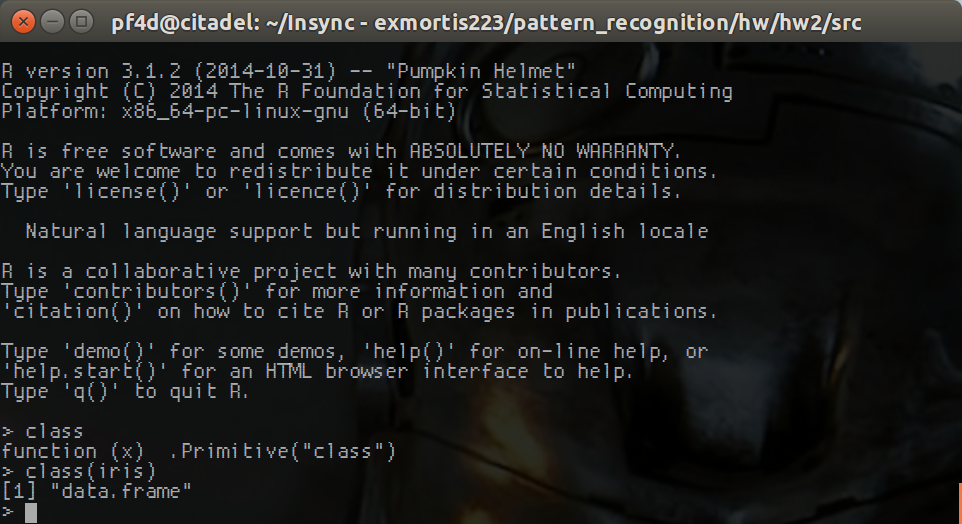
\includegraphics[width=0.45\textwidth]{images/class_command.png}
\end{figure}

\section{\texttt{summary} command :}

The \texttt{summary} command applied to the \texttt{iris} dataset, is a ``generic function used to produce result summaries of the results of various model fitting functions.  The function invokes particular methods which depend on the `class' of the first argument.''

\begin{figure}[H]
  \centering
    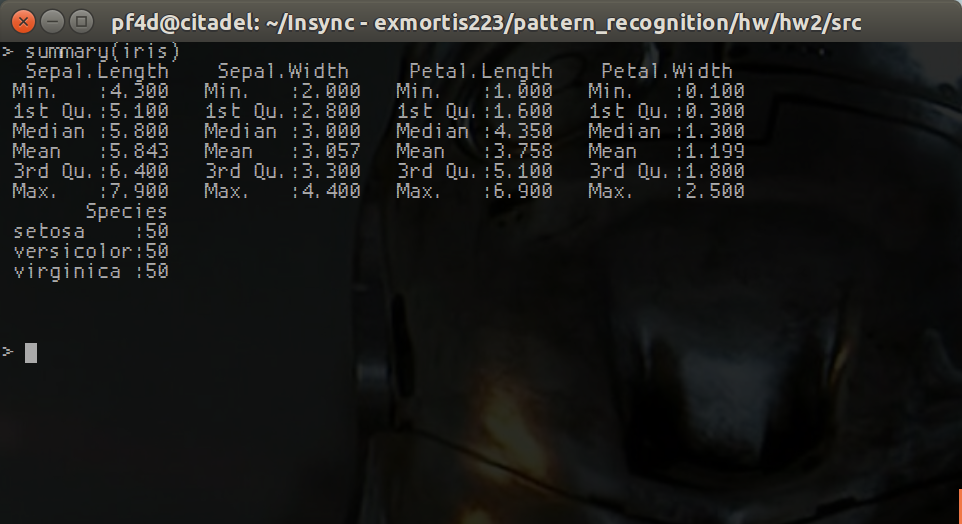
\includegraphics[width=0.45\textwidth]{images/summary_command.png}
\end{figure}

\section{\texttt{labels} command :}

The \texttt{labels} command: ``Find[s] a suitable set of labels from an object for use in printing or plotting.  For example, a generic function.''

\begin{figure}[H]
  \centering
    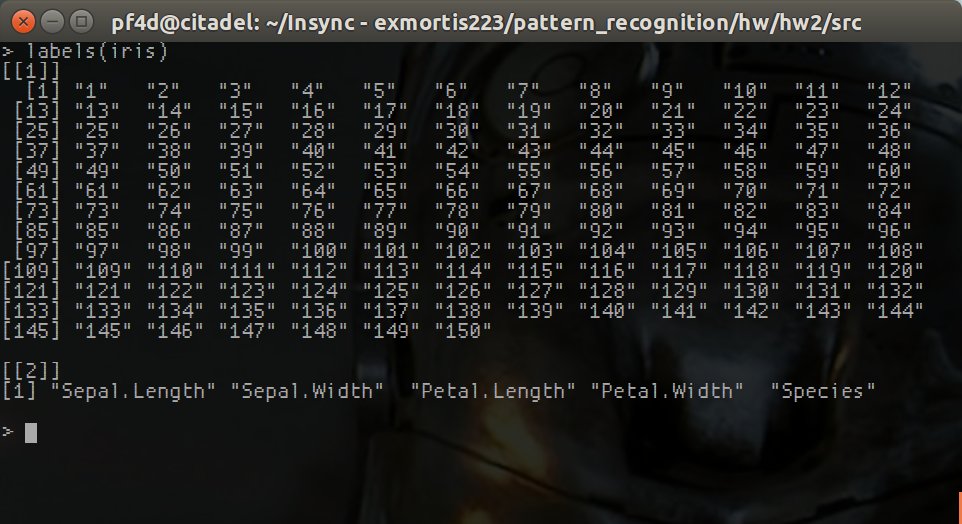
\includegraphics[width=0.45\textwidth]{images/labels_command.png}
\end{figure}

\section{\texttt{colnames} command :}

The \texttt{colnames} command: ``Retrieve[s] or set[s] the row or column names of a matrix-like object.''

\begin{figure}[H]
  \centering
    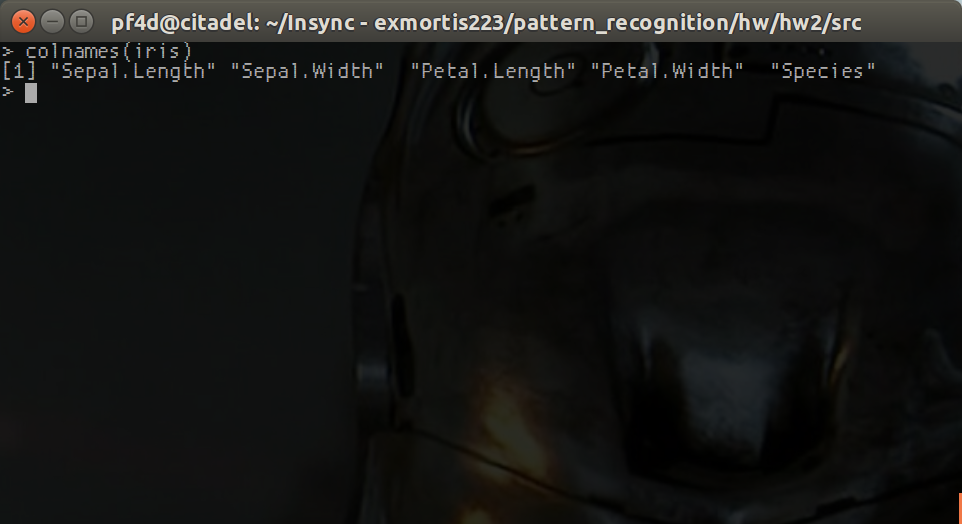
\includegraphics[width=0.45\textwidth]{images/colnames_command.png}
\end{figure}

\section{tab-completion :}

Pressing \texttt{tab} after a \texttt{data.frame} object with accessor-operator \texttt{\$} will provide variable names.

\begin{figure}[H]
  \centering
    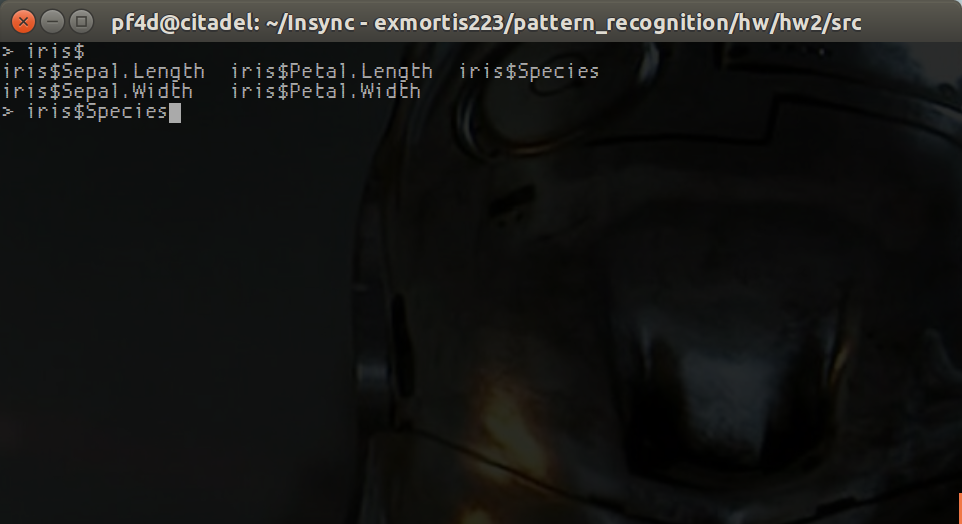
\includegraphics[width=0.45\textwidth]{images/tab_completion.png}
\end{figure}

\section{Iris data PCA plotting :}

\begin{figure}[H]
  \centering
    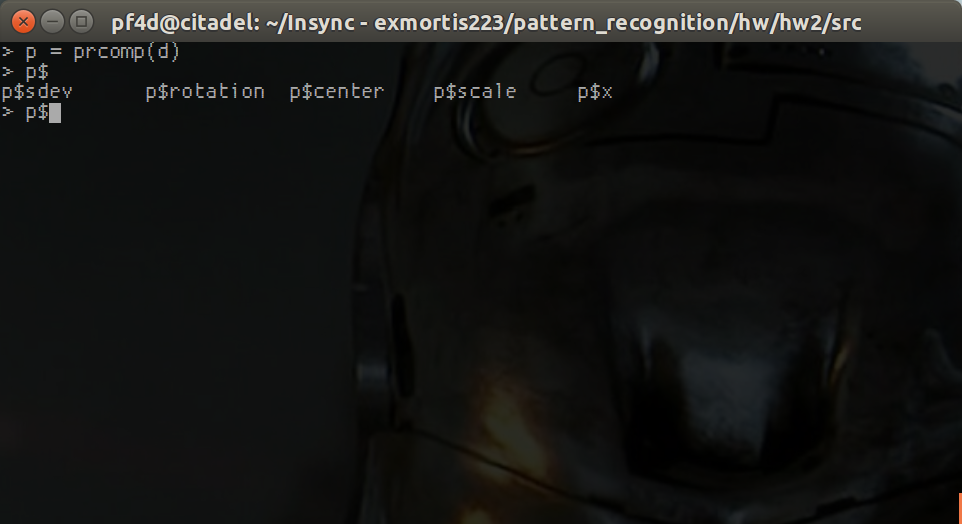
\includegraphics[width=0.45\textwidth]{images/prcomp_tab.png}
\end{figure}

\begin{figure}[H]
  \centering
    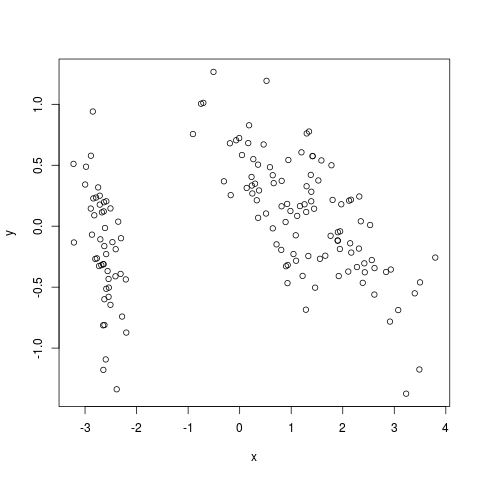
\includegraphics[width=0.45\textwidth]{images/pca_plot.png}
  \caption{PCA-plot showing what appears to be two clusters, despite the fact that there are three distinct species of iris.}
\end{figure}

The \texttt{plot} command, a ``Generic function for plotting of R objects.  For more details about the graphical parameter arguments, see `par'.

For simple scatter plots, \texttt{plot.default} will be used.  However, there are \texttt{plot} methods for many R objects, including \texttt{function}'s, \texttt{data.frame}'s, \texttt{density} objects, etc.  Use \texttt{methods(plot)} and the documentation for these.''

\begin{figure}[H]
  \centering
    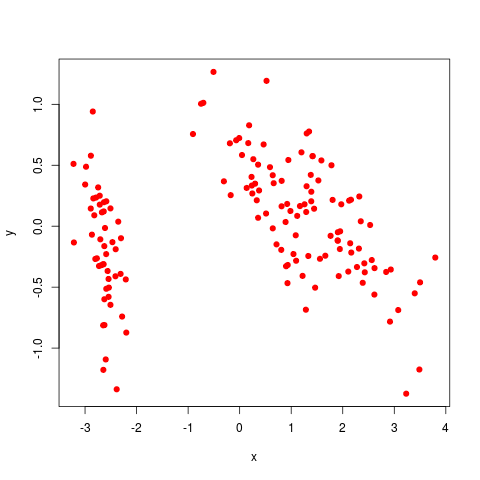
\includegraphics[width=0.45\textwidth]{images/pca_plot_red.png}
\end{figure}

\begin{figure}[H]
  \centering
    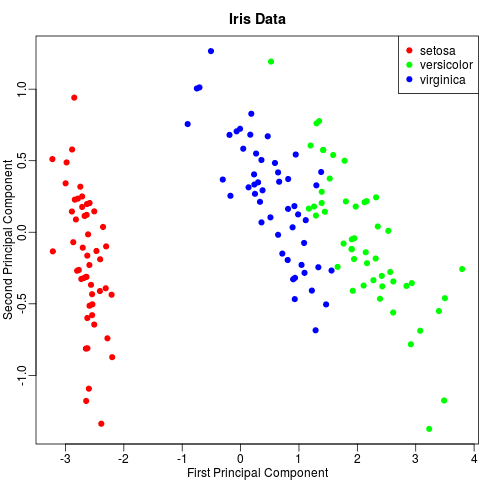
\includegraphics[width=0.35\textwidth]{images/pca_plot_class.png}
\end{figure}

\begin{figure}[H]
  \centering
    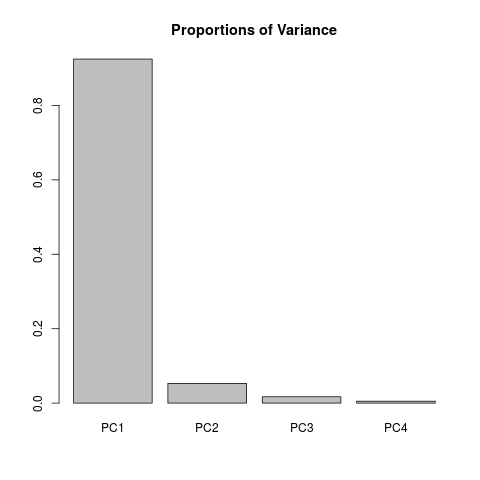
\includegraphics[width=0.45\textwidth]{images/pca_pvar_barplot.png}
\end{figure}

\subsection{Source code :}

\begin{Rs}
# store the iris 'classes' :
c = iris[,5]

# store the iris 'data' :
d = iris[,seq(1,4)]

# perform PCA on d :
p = prcomp(d)

# set the 1st principle component :
x = p$x[,1]

# set the 2nd principle component :
y = p$x[,2]

# plot them :
png('../doc/images/pca_plot.png')
plot(x,y)
dev.off()

# plot them in red :
png('../doc/images/pca_plot_red.png')
plot(x,y, col='red', bg='red', type='p', pch=21)
dev.off()

# store indexes of classes :
s  = which(c == 'setosa')
vc = which(c == 'versicolor')
vg = which(c == 'virginica')

# color vector :
cc     = as.vector(c)
cc[s]  = 'red'
cc[vc] = 'blue'
cc[vg] = 'green'

# plot them colored by class :
png('../doc/images/pca_plot_class.png')
X11(width=4, height=4)
par(mar=c(2.5,2.5,2.5,.1),mgp = c(1.5, .5, 0))
plot(x,y, col=cc, bg=cc, type='p', pch=21, xlab='First Principal Component',
     ylab='Second Principal Component', main='Iris Data')
legend('topright', levels(c),
       col   = c('red', 'green', 'blue'), 
       pt.bg = c('red', 'green', 'blue'), pch = 21)
dev.off()

# do a barplot of the proportions of variance :
sig  = p$sdev**2
pvar =  sig / sum(sig)
png('../doc/images/pca_pvar_barplot.png')
barplot(pvar, names.arg=c('PC1','PC2','PC3','PC4'),
        main='Proportions of Variance')
dev.off()
\end{Rs}

\section{Fruit data :}

While the iris data appears to be highly grouped, the fruit data appears much less so.  However, the lemons seem to be clustered distintly from the other fruit.  Therefore, I believe that these data \emph{do} show enough structure for machine learning techniques; with apples, oranges, and peaches potentially presenting the highest challenge.

\begin{figure}[H]
  \centering
    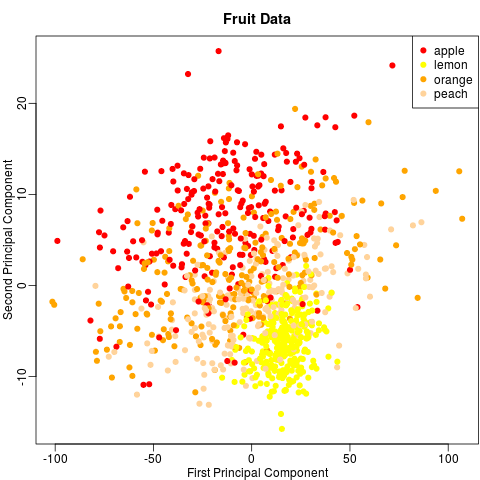
\includegraphics[width=0.45\textwidth]{images/pca_plot_fruit.png}
\end{figure}

\begin{figure}[H]
  \centering
    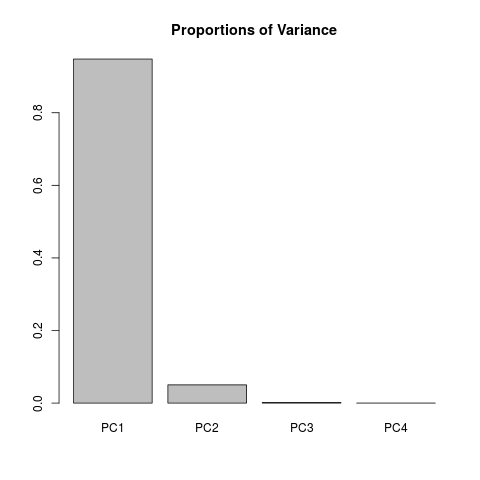
\includegraphics[width=0.45\textwidth]{images/pca_pvar_fruit_barplot.png}
  \caption{The proportions of the variance in the fruit data.  The principle component captures $\approx$ 94\% of the variation.}
\end{figure}

\begin{figure}[H]
  \centering
    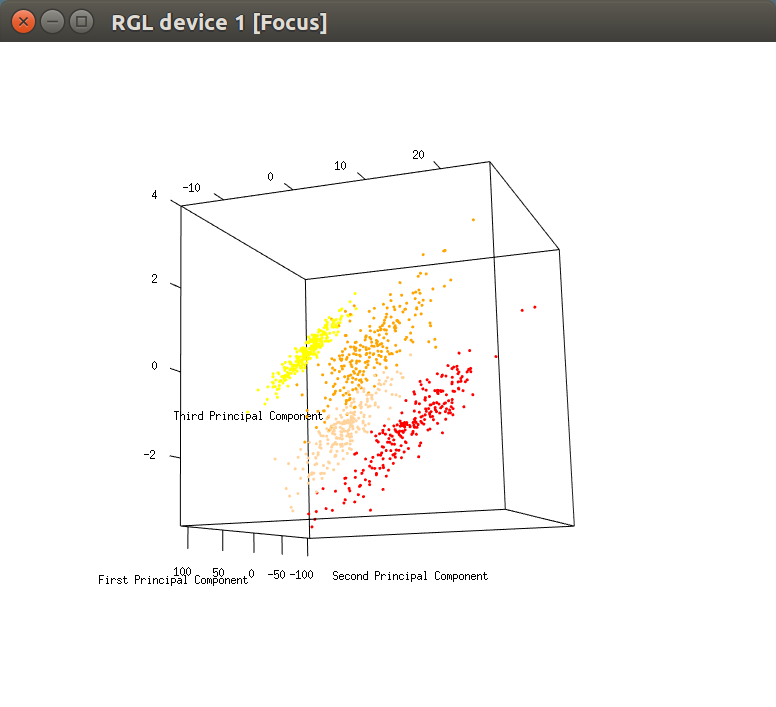
\includegraphics[width=0.45\textwidth]{images/fruit_3d.png}
  \caption{In 3D, we can see much more distinct clustering.}
\end{figure}

\begin{figure}[H]
  \centering
    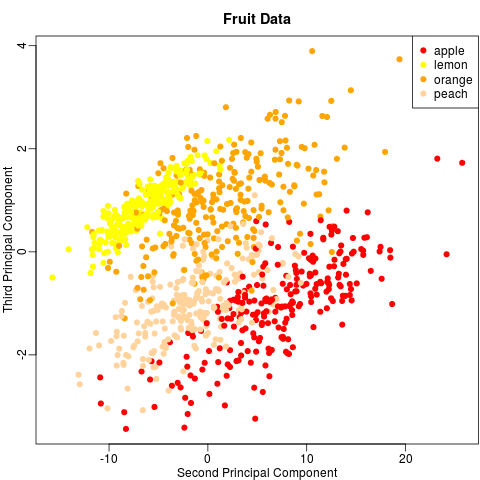
\includegraphics[width=0.45\textwidth]{images/pca_plot_fruit_23.png}
  \caption{The second and third principle components, highlighting the clustering nature of the fruit data.}
\end{figure}

\subsection{Source code :}
\begin{Rs}
# read the variable back in :
f = read.csv("../data/fruit.csv")

# store the fruit 'classes' :
c = f[,5]

# store the fruit 'data' :
d = f[,seq(1,4)]

# perform PCA on d :
p = prcomp(d)

# set the 1st principle component :
x = p$x[,1]

# set the 2nd principle component :
y = p$x[,2]

# set the 3nd principle component :
z = p$x[,3]

# store indexes of classes :
a = which(c == 'apple')
l = which(c == 'lemon')
o = which(c == 'orange')
z = which(c == 'peach')

# color vector :
cols  = c('red', 'yellow', 'orange', 'burlywood1')
cc    = as.vector(c)
cc[a] = cols[1]
cc[l] = cols[2]
cc[o] = cols[3]
cc[z] = cols[4]

# plot them colored by class :
png('../doc/images/pca_plot_fruit.png')
#X11(width=4, height=4)
par(mar=c(2.5,2.5,2.5,.1),mgp = c(1.5, .5, 0))
plot(x,y, col=cc, bg=cc, type='p', pch=21, xlab='First Principal Component',
     ylab='Second Principal Component', main='Fruit Data')
legend('topright', levels(c), col = cols, pt.bg = cols, pch = 21)
dev.off()

# do a barplot of the proportions of variance :
sig  = p$sdev**2
pvar =  sig / sum(sig)
png('../doc/images/pca_pvar_fruit_barplot.png')
barplot(pvar, names.arg=c('PC1','PC2','PC3','PC4'),
        main='Proportions of Variance')
dev.off()

# import the rgl library for 3D stuff:
library(rgl)

plot3d(x,y,z, col=cc, bg=cc, type='p', pch=21,
       xlab='First Principal Component',
       ylab='Second Principal Component',
       zlab='Third Principal Component')

# plot them colored by class :
png('../doc/images/pca_plot_fruit_23.png')
#X11(width=4, height=4)
par(mar=c(2.5,2.5,2.5,.1),mgp = c(1.5, .5, 0))
plot(y,z, col=cc, bg=cc, type='p', pch=21, xlab='Second Principal Component',
     ylab='Third Principal Component', main='Fruit Data')
legend('topright', levels(c), col = cols, pt.bg = cols, pch = 21)
dev.off()
\end{Rs}


\end{multicols*}

%\begin{figure}[H]
%  \centering
%    \includegraphics[width=0.45\textwidth]{images/.png}
%\end{figure}


\end{document}


